\documentclass[tikz, border=1mm]{standalone}
\usepackage{tikz} 
\usetikzlibrary{arrows.meta}
\usepackage{pgfplots}

\pgfplotsset{compat=1.18}

\begin{document}

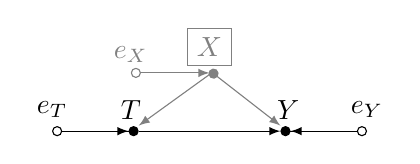
\begin{tikzpicture}

    % dag_bb3
    \node at (-2,0) {$e_{T}$};
    \node at (-1,0) {$T$};
    \node[gray] at (-1,0.7) {$e_{X}$};
    \node[rectangle,draw,gray] at (0,0.8) {$X$};
    \node at (1,0) {$Y$};
    \node at (2,0) {$e_{Y}$};

    \draw[{Circle[open]}-{latex}{Circle}](-2,-0.27) to (-0.9,-0.27); % eT -> T (circle)
    \draw[-{latex},gray](0,0.45) to (-0.9,-0.2); % X -> T
    \draw[{Circle[open]}-{latex},gray](-1,0.47) to (0,0.47); % eX -> X (circle)
    \draw[-{latex}](-0.9,-0.27) to (0.9,-0.27); % T -> Y
    \draw[{Circle}-{latex},gray](0,0.5) to (0.9,-0.2); % X -> Y
    \draw[{Circle[open]}-{latex}{Circle}](2,-0.27) to (0.9,-0.27); % eY -> Y (circle)
    
\end{tikzpicture}

\end{document}
